\documentclass[12pt]{article}

%packages
\usepackage{fancyhdr}
\usepackage[margin=1in]{geometry}
\usepackage[utf8]{inputenc}
\usepackage{listings}
\usepackage{booktabs}
\usepackage{enumitem}
\usepackage{pdfpages}
\usepackage{graphicx}
\usepackage{listings}
\usepackage{xcolor}
\usepackage{subcaption}
\usepackage{float}
\usepackage{amsmath}

%fancyheadr fix
\setlength{\headheight}{15pt}

%commands to lslistings
\lstset{
    basicstyle=\ttfamily\small,
    breaklines=true,     
    breakatwhitespace=true,
    frame=single,
    numbers=left,
    numberstyle=\tiny,
    columns=fullflexible,
    keepspaces=true
}


%title info
\newcommand{\doctitle}{STA 5635 HW 2}
\newcommand{\name}{Palmer Swanson}

\pagestyle{fancy}
\lhead{\textbf{\doctitle}}
\chead{\name}
\rhead{\today}

%document
\begin{document}

\section*{Problem 1}
\begin{itemize}
    \item Need to minimize the following:
    \[
    C(\boldsymbol{\omega}) = -\frac{1}{N}L(\boldsymbol{\omega}) + \lambda\boldsymbol{\omega}^T\boldsymbol{\omega}
    \]
    where 
    \[
    L(\omega) = \sum_{j=1}^{n}y_j(w_0 + \sum_{i=1}^{p}w_ix_{ji}) - ln(1+ exp(w_0 + \sum_{i=1}^{p}w_ix_{ji}))
    \]
    We minimize this loss using gradient descent, using:
    \[
    \boldsymbol{w}^{t+1}\leftarrow \boldsymbol{\omega}^{t} - \eta\lambda\boldsymbol{\omega}^{t} + 
    \frac{\eta}{N}\frac{\partial L(\boldsymbol{\omega}^{t})}{\partial \boldsymbol{\omega}}
    \]

    According to the notes, we basically do an Odds ratio decision rule:

    \begin{table}[htbp]
        \centering
        \input{../output/logreg_misclass_table.tex}
        \caption{Best learning rate $\eta$, training and test misclassification error, Logistic Regression.}
        \label{tab:logreg_misclass}
    \end{table}
\end{itemize}

\section*{Problem 2}
We need to minimize analytically:
    \[
    C(\boldsymbol{\omega}) = \frac{1}{N}\sum_{i=1}^{n}\left(y_i - 
    \boldsymbol{\omega}^T\boldsymbol{x}_i - \omega_0\right)^2 + 
    \lambda\left(\boldsymbol{\omega}^T\boldsymbol{\omega} + \omega_0^2\right)
    \]
    where $\lambda$ = 0.001, $(\boldsymbol{x_i}, y_i)$ are the training data, and \(y_i\in\{-1,+1\}\).
    Predict classification via \(\hat{y} = \text{sign}(\boldsymbol{\omega}^T\boldsymbol{x} + \omega_0)\).
\begin{itemize}
    \item We can report the misclassification error of the training and test datasets in the following table:
    \begin{table}[htbp]
        \centering
        \input{../output/q2_table.tex}
        \caption{misclassification Error for training and test datasets, Ridge like regression}
        \label{tab:ridge_classification}
    \end{table}

    The train misclassification error rate is the same (0.00), though the test error rate is
    higher (0.091 vs. 0.020).
    \item We can display the ROC curve for both the ridge and logistic models in figure \ref{fig:q2_roc}.
    \begin{figure}[htbp]
        \centering
        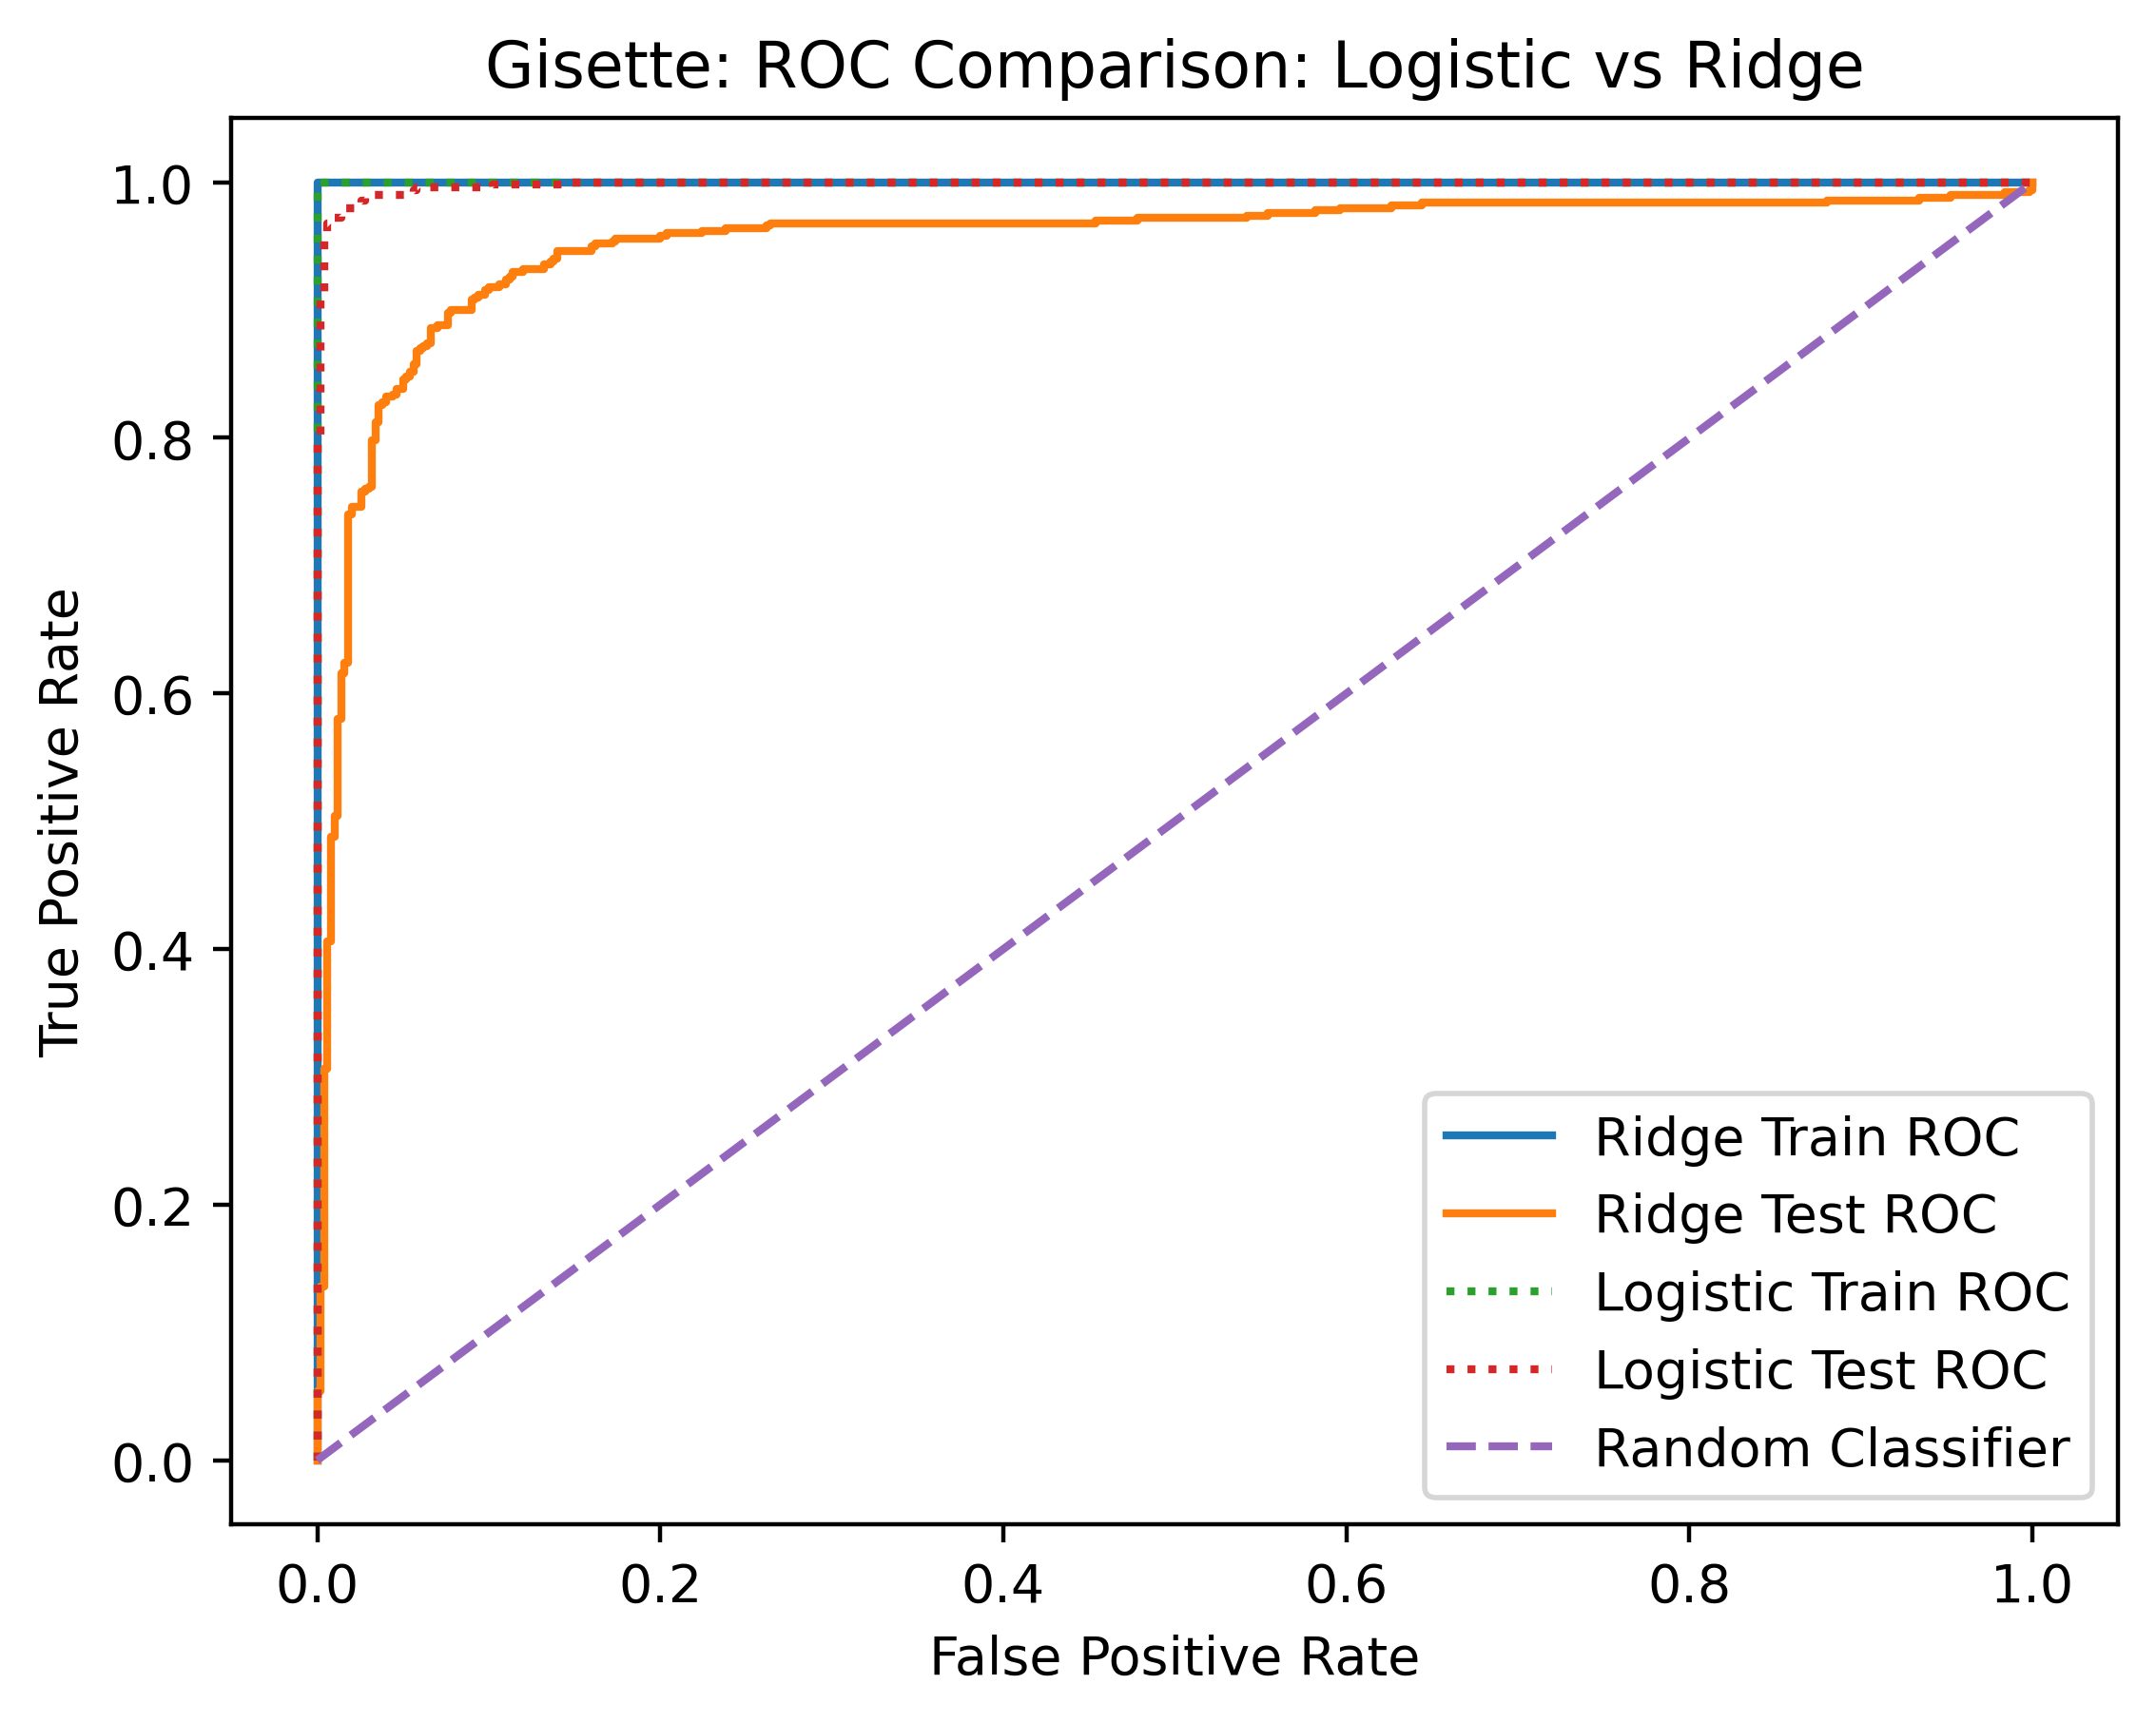
\includegraphics[totalheight=7cm]{../figures/q2_roc_plot.png}
        \caption{Average log determinant vs Lambda.}
        \label{fig:q2_roc}
    \end{figure}

    The train ROC for the logistic and ridge models are practically the same.  The ROC for the logistic model
    is better than the ridge though; tighter to the upper left hand corner.  
\end{itemize}

\end{document}